\begin{problem}{Лесенки}{стандартный ввод}{стандартный вывод}{1 секунда}{256 мегабайт}

Лесенкой называется набор кубиков в один или несколько слоёв, в котором
каждый более верхний слой содержит кубиков меньше, чем нижний.

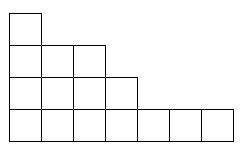
\includegraphics[scale=1,natwidth=243, natheight=152]{lesenki_image_ru_1.jpg}

Подсчитать число лесенок, которое можно построить из $N$ кубиков.


\InputFile
На входе записано число $N$ ($1 \le N \le 200$).


\OutputFile
Вывести искомое число лесенок.

\Example

\begin{example}
\exmp{3
}{2}%
\end{example}

\end{problem}

